\begin{frame}
\frametitle{History of Autonomous Vehicles Development}
\framesubtitle{The Early Years (1990s)}
\begin{columns}[T]
    \begin{column}{.5\textwidth}
    \centering
    Prometheus Project \\
    \vspace{0.25cm}
    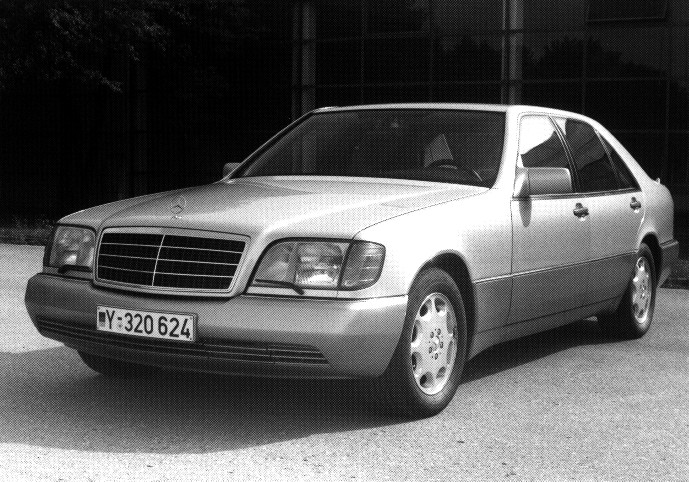
\includegraphics[height=2.2cm]{images/vamp.jpg} \\
    \tiny{\cite{Dickmanns1994} VaMP}
    \footnotesize
    \begin{itemize}
        \item European R\&D project (1985 - 1995)
        \item Prof. Ernst Dickmann's research vehicles
            demonstrated 1,000+ km automated highway drives
    \end{itemize}
    \end{column}
    \pause
    \begin{column}{.5\textwidth}
    \centering
    Demo '97 \\
    \vspace{0.25cm}
    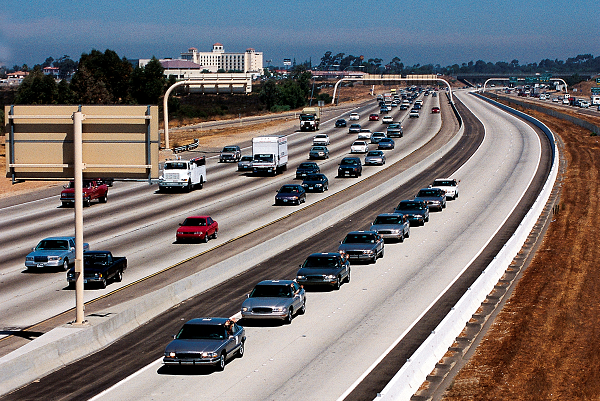
\includegraphics[height=2.2cm]{images/demo-97-no-hands.png} \\
    \tiny{Platoon demo}\footnotemark[1]
    \footnotesize
    \begin{itemize}
        \item US DOT sponsored research to demonstrate the
            Automated Highway System (AHS)
        \item A 12 km stretch of an HOV lane was used for the demonstration
    \end{itemize}
    \end{column}
\end{columns}
\pause
\footnotesize
\begin{block}{}
These projects set the foundation for OEM ADAS development in the
2000s
\end{block}
\footnotetext[1]{\tiny{\url{https://path.berkeley.edu/research/connected-and-automated-vehicles/national-automated-highway-systems-consortium}}}
\end{frame}

\begin{frame}
\frametitle{History of Autonomous Vehicles Development}
\framesubtitle{The DARPA Challenges (2004-2008)}
\begin{columns}[T]
    \begin{column}{.65\textwidth}
    DARPA Grand Challenges\footnotemark[1]
    \begin{itemize}
        \item In the 2004 competition, 15 teams competed for a \$1 million prize
            on a 240 km desert route
        \item The prize went unclaimed; the best team was able to complete
            11.78 km
        \item In 2005, a \$2 million prize was up for grabs on a 212 km route
        \item The team from Stanford University with their vehicle
            \emph{Stanley} completed the course the fastest (in total 5 teams
            completed the course)
    \end{itemize}
    \end{column}
    \begin{column}{.35\textwidth}
    \centering
    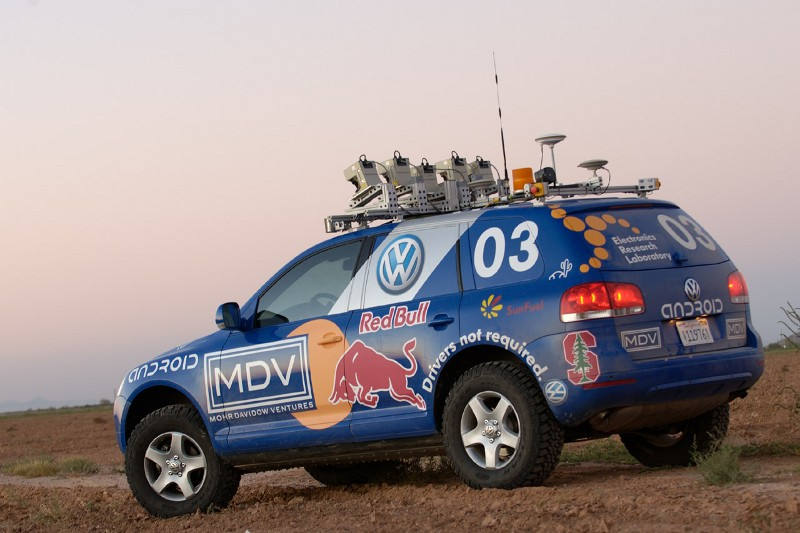
\includegraphics[height=3cm]{images/darpa_stanley.jpg} \\
    \tiny{\cite{DARPAStanley}}
    \end{column}
\end{columns}
\footnotetext[1]{\tiny{\url{https://www.darpa.mil/about-us/timeline/-grand-challenge-for-autonomous-vehicles}}}
\end{frame}
    
\begin{frame}
\frametitle{History of Autonomous Vehicles Development}
\framesubtitle{The DARPA Challenges (2004-2008)}
\begin{columns}[T]
    \begin{column}{.6\textwidth}
    DARPA Urban Challenge\footnotemark[1]
    \begin{itemize}
        \item In 2007, a third competition for a \$2 million prize was held on
            a 96 km urban route
        \item A total of 11 teams competed in the final competition
        \item A team from Carnegie Melon University won with their vehicle
            \emph{Boss}
    \end{itemize}
    \end{column}
    \begin{column}{.4\textwidth}
    \centering
    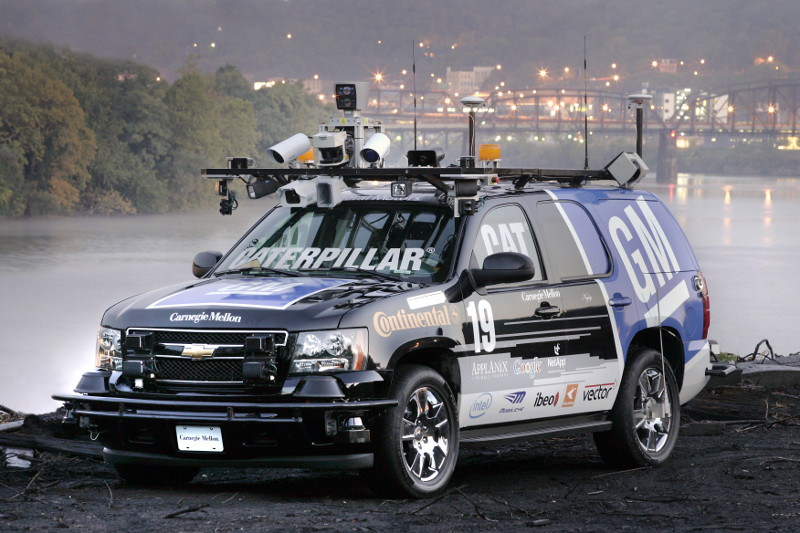
\includegraphics[height=3cm]{images/darpa_boss.jpg} \\
    \tiny{\cite{CMUUrbanChallenge}}
    \end{column}
\end{columns}
\pause
\vspace{0.25cm}
\begin{block}{}
The student, engineers, and companies of the DARPA challenges laid the
foundations for today's autonomous driving development and are leaders in the
industry.
\end{block}
\footnotetext[1]{\tiny{\url{https://www.darpa.mil/about-us/timeline/darpa-urban-challenge}}}
\end{frame}

\begin{frame}
\frametitle{History of Autonomous Vehicles Development}
\framesubtitle{The Industry Ramp-Up Phase (2010-2020)}
\centering OEMs and Tier 1s
\begin{columns}[T]
    \begin{column}{.25\textwidth}
        \centering
        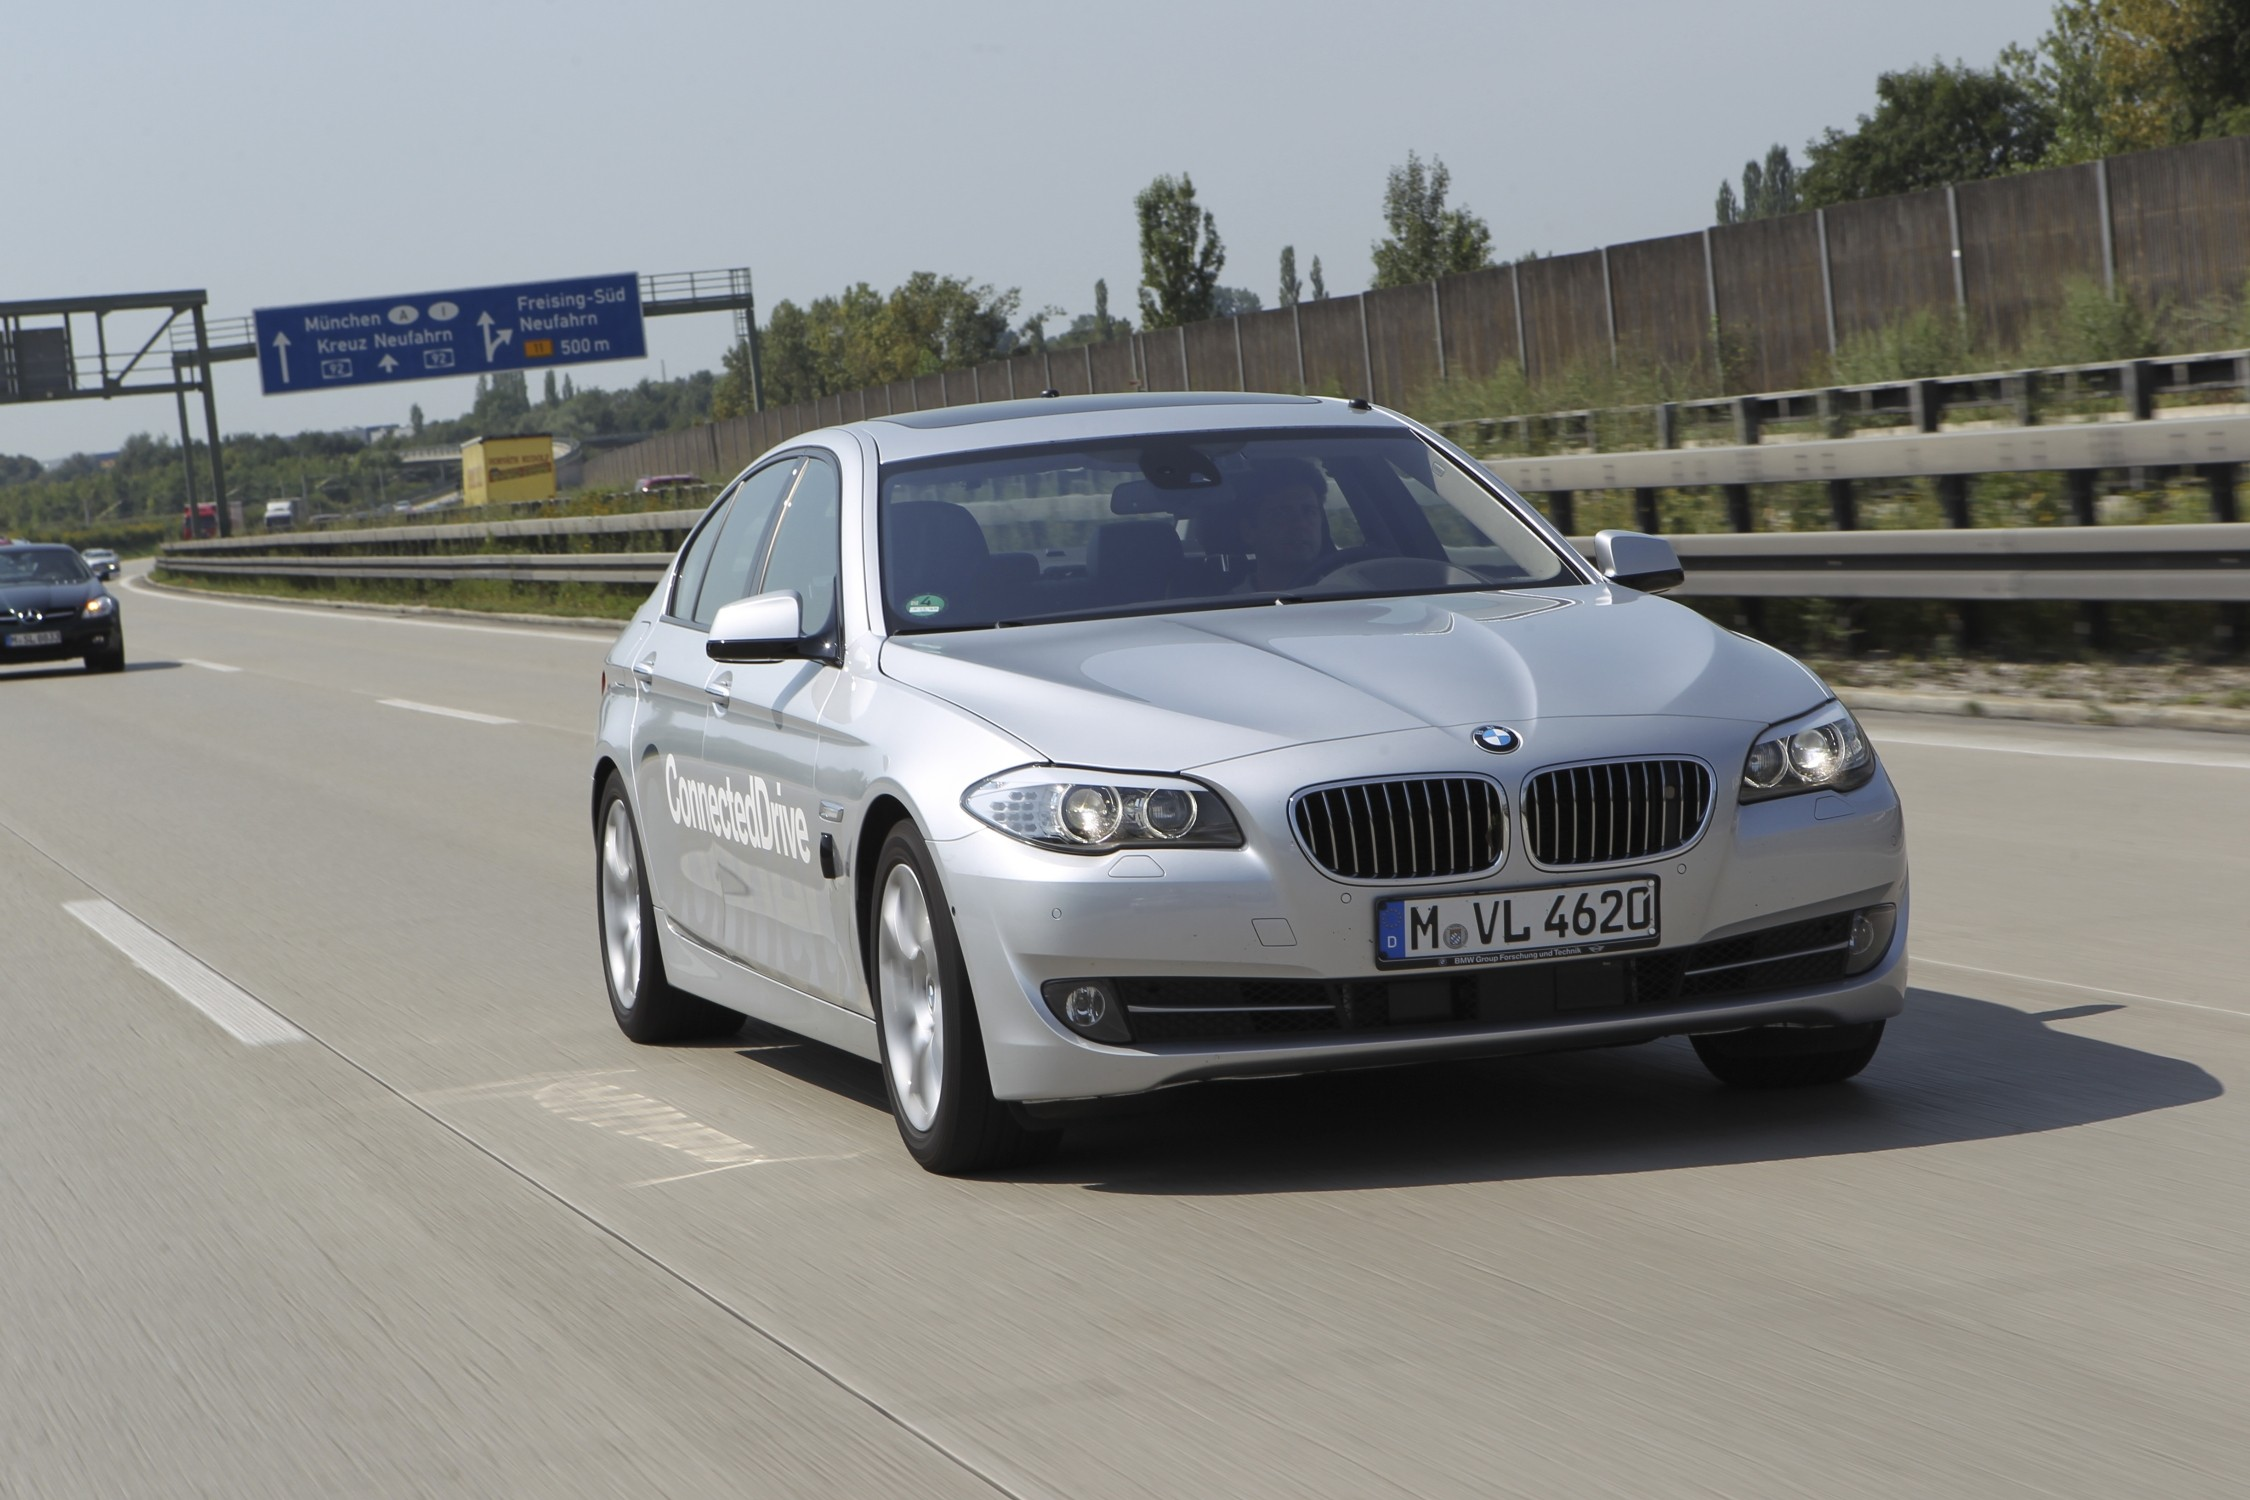
\includegraphics[height=1.9cm]{images/bmw_had.jpg} \\
        \footnotesize BMW \cite{AeberhardBMWHAF2015}
    \end{column}
    \begin{column}{.25\textwidth}
        \centering
        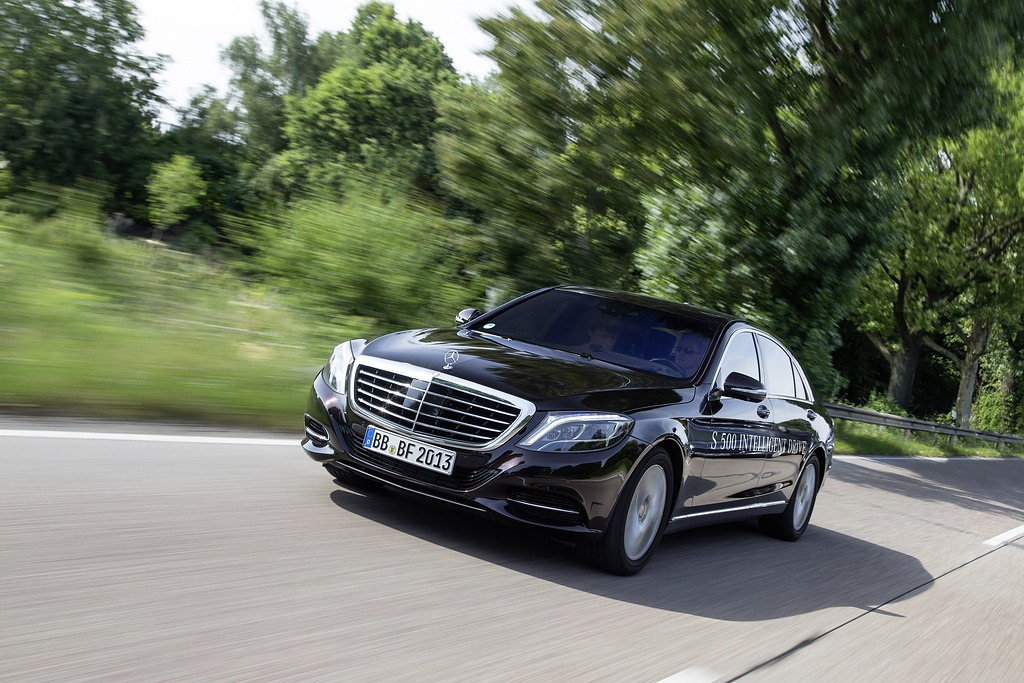
\includegraphics[height=1.9cm]{images/mercedes_bertha_benz_drive.jpg} \\
        \footnotesize Mercedes-Benz \cite{DaimlerBertha2014}
    \end{column}
    \begin{column}{.25\textwidth}
        \centering
        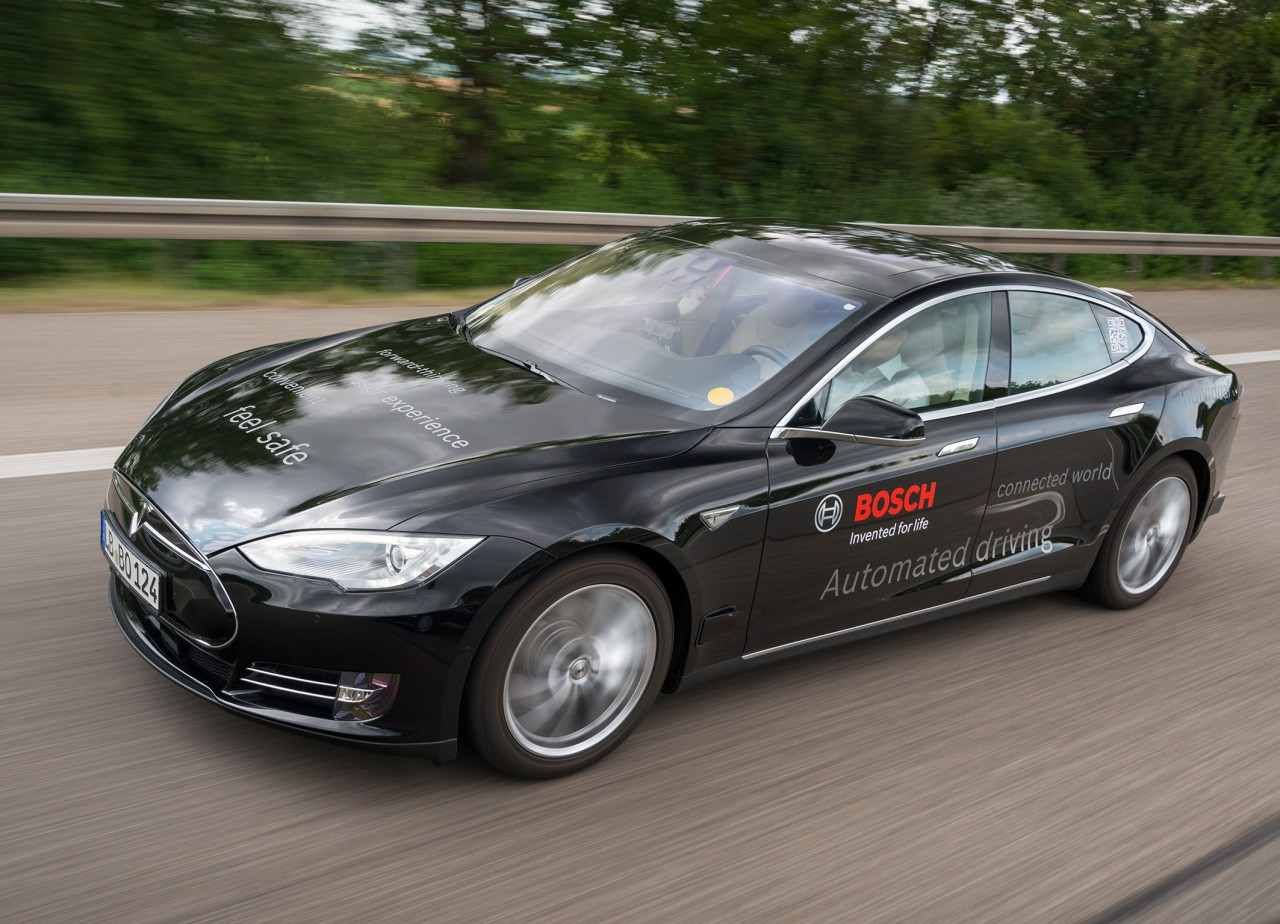
\includegraphics[height=1.9cm]{images/bosch_had.jpg} \\
        \footnotesize Bosch \cite{BoschPressHAD}
    \end{column}
    \begin{column}{.25\textwidth}
        \centering
        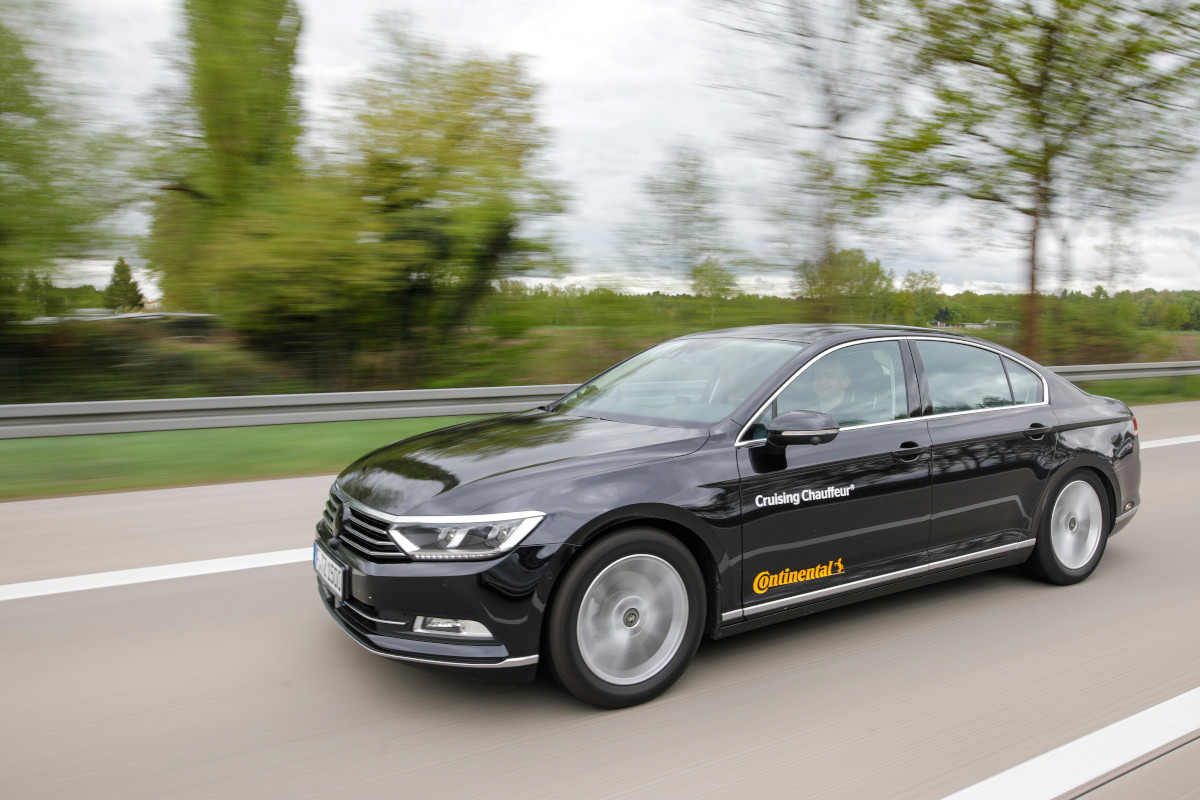
\includegraphics[height=1.9cm]{images/continental_had.jpg} \\
        \footnotesize Continental \cite{ContinentalHAD}
    \end{column}
\end{columns}
\vspace{0.5cm}
\centering New Players
\begin{columns}[T]
    \begin{column}{.25\textwidth}
        \centering
        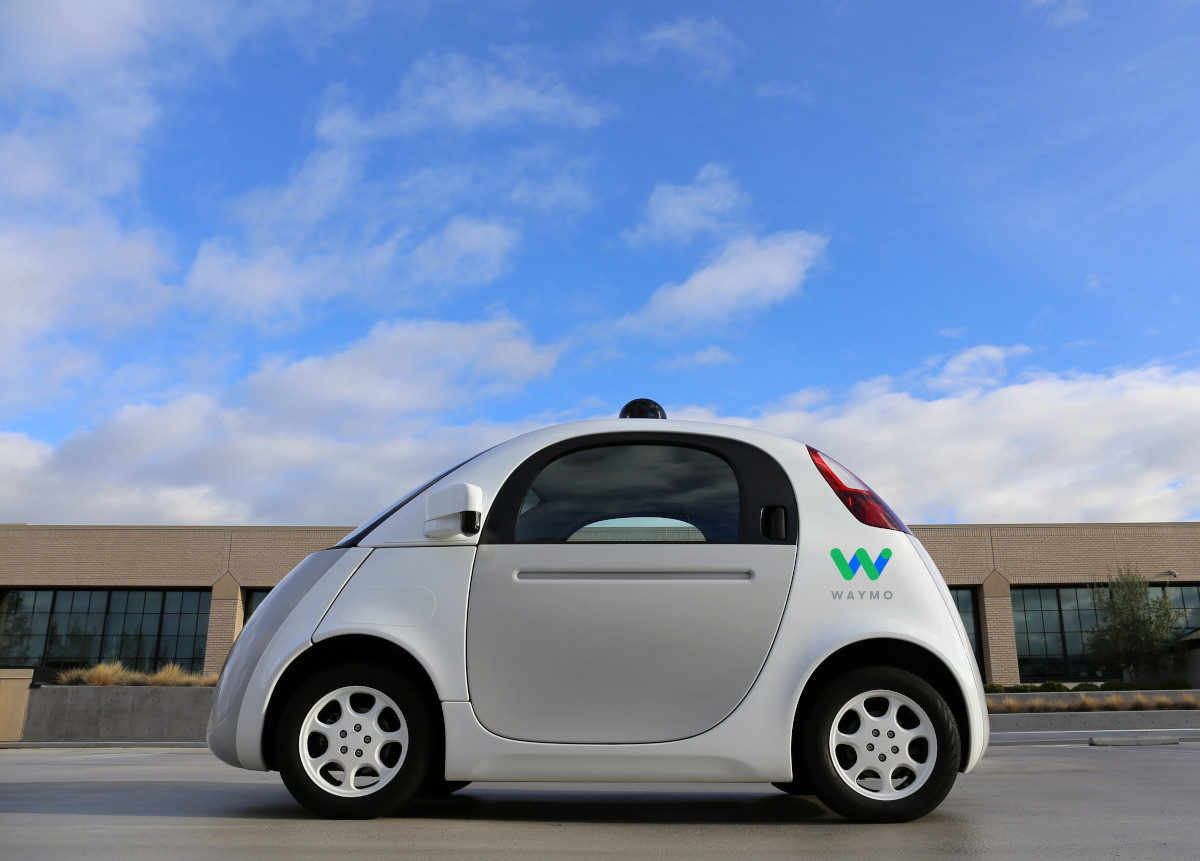
\includegraphics[height=1.9cm]{images/waymo_firefly.jpg} \\
        \footnotesize Waymo \cite{WaymoPress}
    \end{column}
    \begin{column}{.25\textwidth}
        \centering
        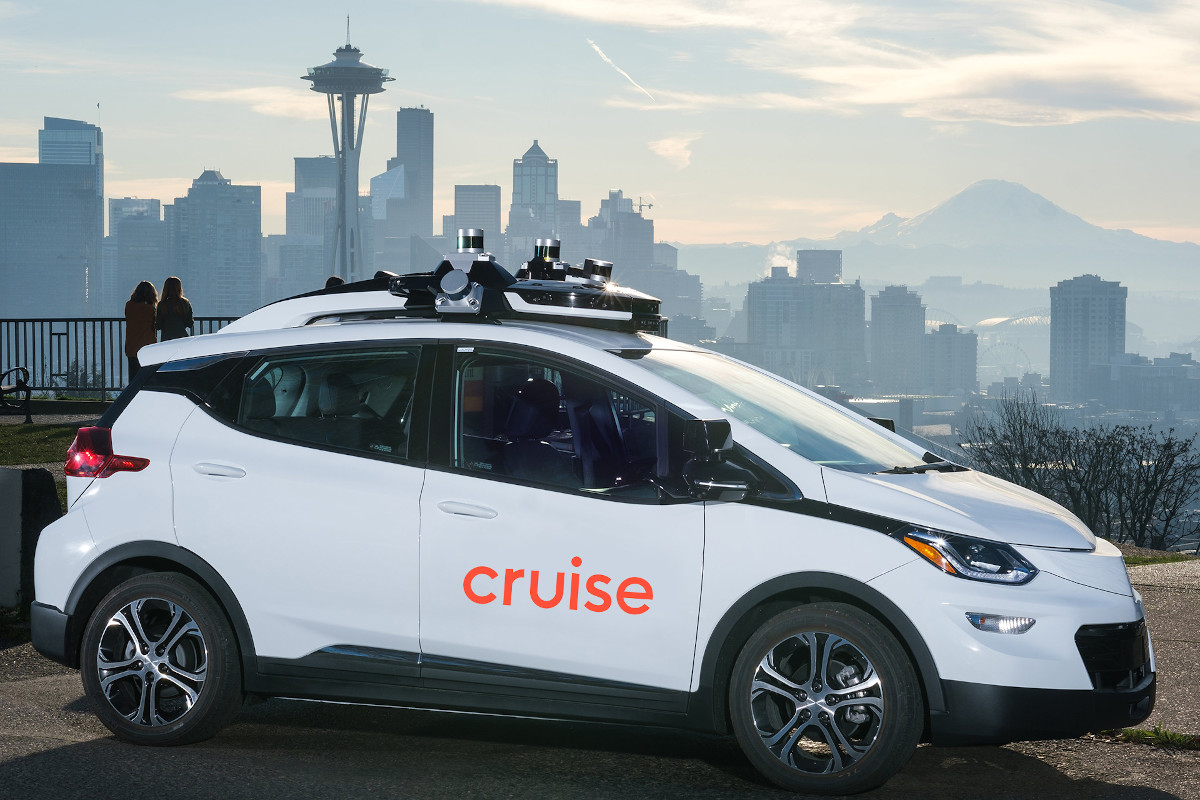
\includegraphics[height=1.9cm]{images/cruise_vehicle.jpg} \\
        \footnotesize Cruise \cite{CruiseNews}
    \end{column}
    \begin{column}{.25\textwidth}
        \centering
        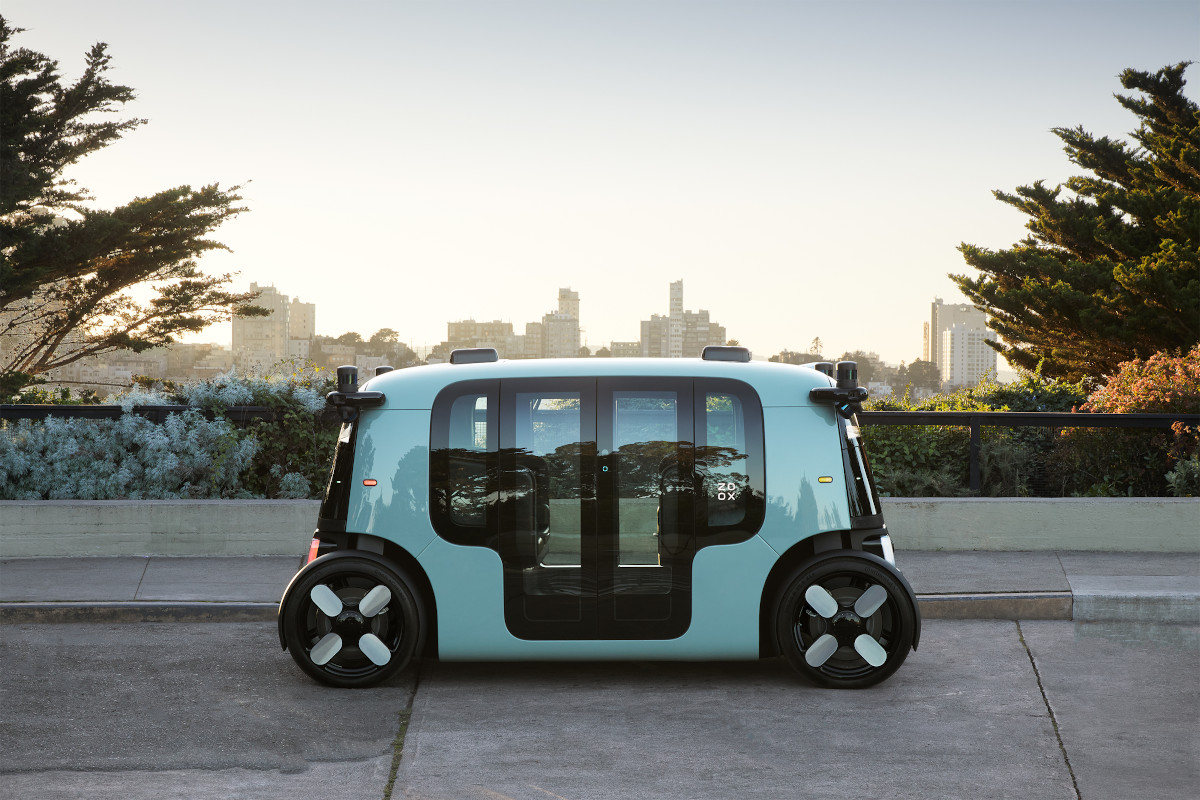
\includegraphics[height=1.9cm]{images/zoox_vehicle.jpg} \\
        \footnotesize Zoox \cite{ZooxPress}
    \end{column}
    \begin{column}{.25\textwidth}
        \centering
        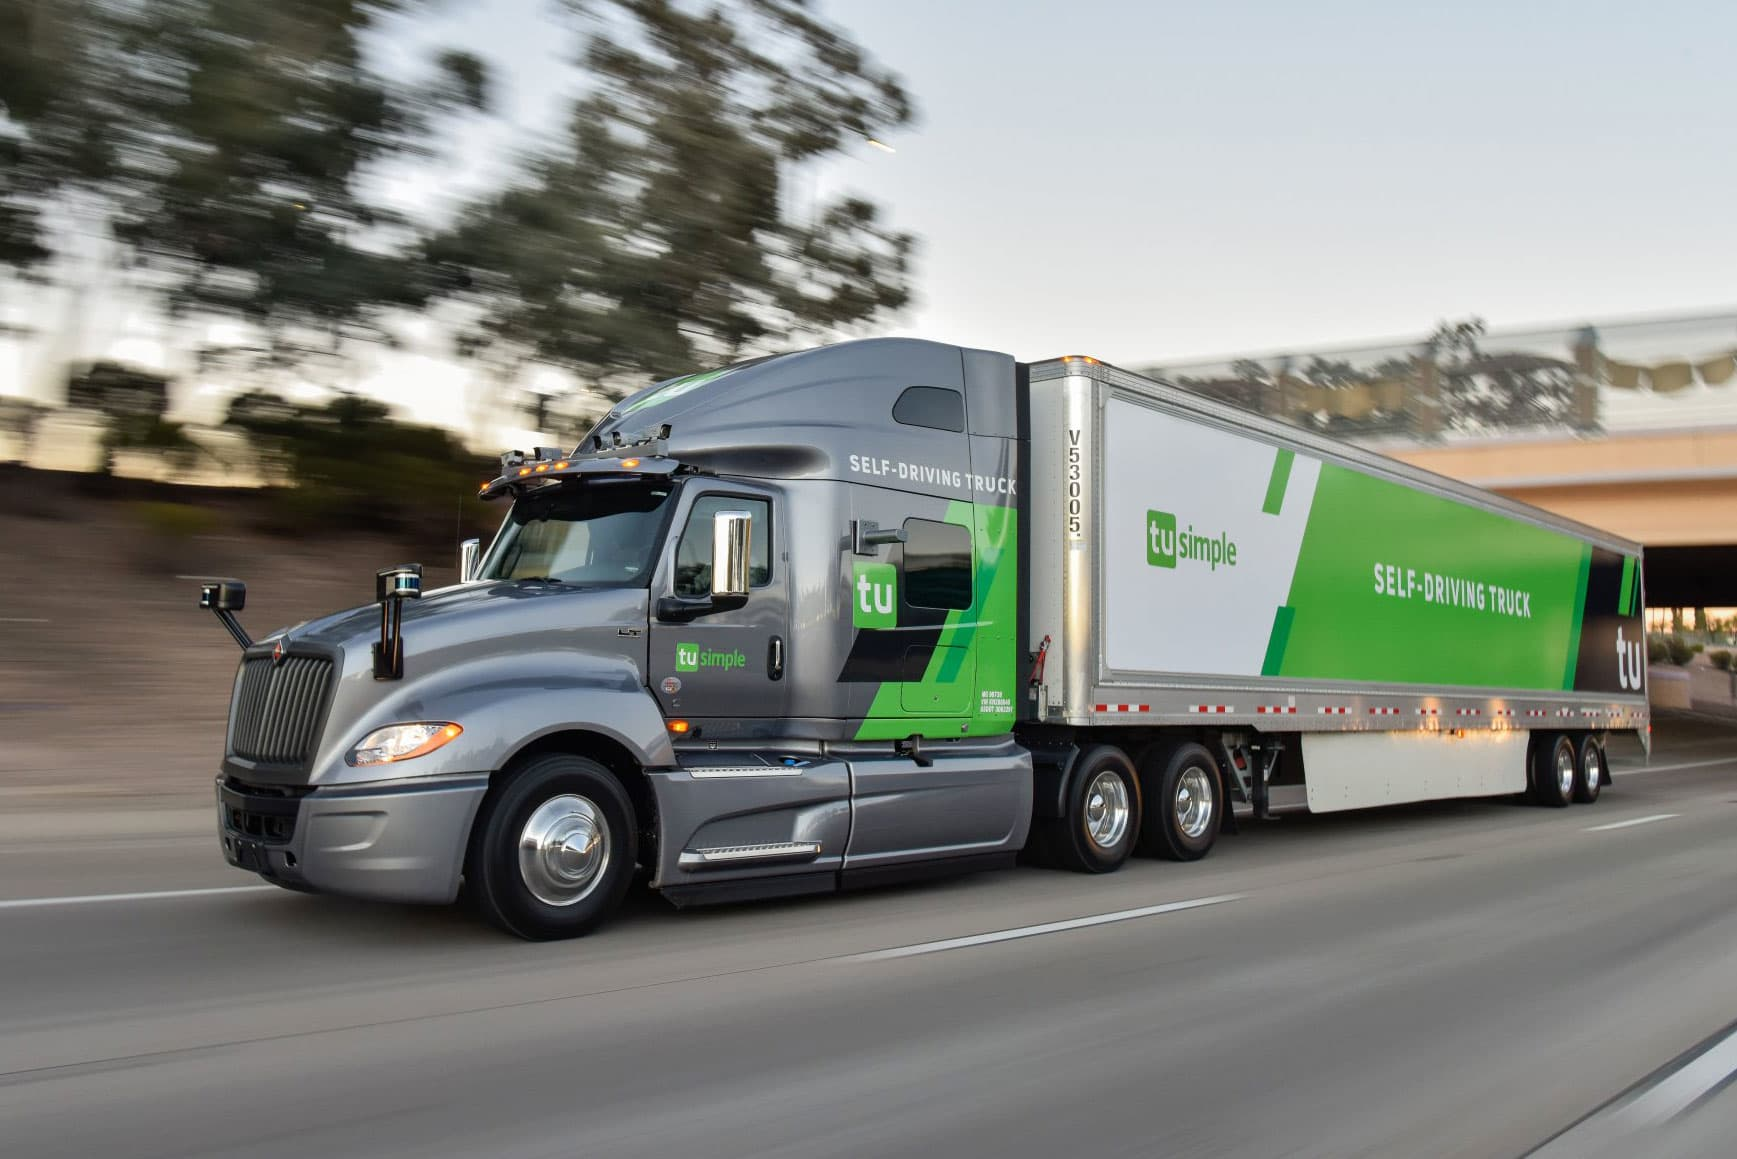
\includegraphics[height=1.9cm]{images/tusimple_vehicle.jpg} \\
        \footnotesize TuSimple \cite{TuSimpleMedia}
    \end{column}
\end{columns}
\end{frame}

\begin{frame}
\frametitle{History of Autonomous Vehicles Development}
\framesubtitle{Going to Production (2020 - ???)}
Only since 2020 have the first true driveless vehicles been allowed to operate
on public roads, albeit in limited numbers and locations.\\
\vspace{0.5cm}
Examples: \\
Waymo One, Cruise, Mercedes Level 3
\begin{block}{}
The next decade will be the beginning of the commercialization of autonomous
vehicles. Many challenges remain for widespread adoption...
\end{block}
\end{frame}